\chapter{Experiments and Evaluation}
\label{chap:experiments}

This chapter presents the empirical evaluation of the proposed structural-primitives grammar for grammar-based fuzzing of SQLite. The evaluation is organized around three research questions that address CVE rediscovery effectiveness, general bug detection capability, and performance trade-offs relative to a generic baseline grammar. Section~\ref{sec:rqs} states the research questions. Section~\ref{sec:setup} describes the experimental setup. Section~\ref{sec:baselines} introduces the baseline method. Section~\ref{sec:metrics} defines the evaluation metrics. Section~\ref{sec:results} presents the experimental results. Section~\ref{sec:discussion} provides analysis and discussion.


\section{Research Questions}
\label{sec:rqs}

The evaluation addresses the following three research questions:

\begin{description}
  \item[RQ1 (CVE Rediscovery).] Can the structural-primitives grammar, augmented with low-weight seed rules, reliably rediscover known CVEs in historical SQLite versions?
  \item[RQ2 (Bug Detection).] Does the compositional grammar --- without CVE-specific seed rules --- discover previously unreported bug classes beyond the target CVEs?
  \item[RQ3 (Performance Trade-off).] How does the structural-primitives grammar compare to a generic EBNF baseline in terms of throughput, edge coverage, unique root causes, and time to first crash?
\end{description}

RQ1 measures targeted effectiveness: whether domain-knowledge-driven grammar engineering can reconstruct CVE-triggering inputs from independently encoded structural primitives. RQ2 evaluates generality: whether the same grammar discovers bugs that were not anticipated during grammar design, providing evidence for cross-pollination between structural patterns. RQ3 quantifies the cost of structural complexity: the proposed grammar generates longer, more complex SQL inputs than a generic grammar, and this section measures whether the resulting throughput reduction is offset by improved bug-finding capability.


\section{Dataset and Experimental Setup}
\label{sec:setup}

\subsection{Subjects Under Test}
\label{sec:subjects}

Four SQLite versions with confirmed CVEs served as the primary subjects under test, selected according to three criteria: (1)~\emph{popularity} --- SQLite is the most widely deployed database engine, embedded in virtually all mobile devices, web browsers, and operating systems; (2)~\emph{diversity} --- the four versions span two years of development (2019--2020) and contain six distinct CVEs covering integer overflow, null pointer dereference, use-after-free, and heap buffer overflow bug types; (3)~\emph{reproducibility} --- all versions are publicly available as amalgamation source files, and all target CVEs have published proof-of-concept inputs enabling independent verification.

Table~\ref{tab:subjects} summarizes the subjects under test. Each version was compiled from the SQLite amalgamation (a single C source file of approximately 150{,}000 lines) using Clang~14 with AddressSanitizer (ASan)~\citep{asan} and UndefinedBehaviorSanitizer (UBSan) instrumentation. CVE-2019-19646 was excluded from the rediscovery evaluation because it causes an infinite loop (denial of service) rather than a crash, and the ASan/UBSan oracle cannot detect non-termination within the execution timeout.

\begin{table}[htbp]
\caption{Subjects under test: SQLite versions and associated CVEs.}
\label{tab:subjects}
\centering
\small
\begin{tabular}{llll}
\toprule
\textbf{Version} & \textbf{Release} & \textbf{CVE(s)} & \textbf{Bug Type} \\
\midrule
3.30.1 & 2019-10 & CVE-2019-19646 & Infinite loop (excluded) \\
3.31.1 & 2020-01 & CVE-2020-13434, CVE-2020-9327 & Int overflow, null ptr \\
3.32.0 & 2020-05 & CVE-2020-13435 & Null ptr deref \\
3.32.2 & 2020-06 & CVE-2020-15358, CVE-2020-13871 & Heap overflow, use-after-free \\
\bottomrule
\end{tabular}
\end{table}

\subsection{Seed/Input Dataset}

No external seed corpus was used. The fuzzer generates all inputs from the grammar's production rules, starting from the \texttt{Sql-Stmt} start symbol. The grammar's pre-loaded schema provides the database context: three regular tables (\texttt{t1}, \texttt{t2}, \texttt{t3}), one FTS3 virtual table (\texttt{fts\_t1}), two indices, and one view. This schema is compiled into the harness binary and loaded before each fuzzing execution, ensuring that generated SQL statements operate on a consistent and non-trivial database state.

\subsection{Environment}
\label{sec:environment}

All experiments were conducted on a workstation equipped with an Intel Core i7 processor, 16~GB of RAM, and running Ubuntu 22.04 LTS. The fuzzer was compiled with Rust 1.77 in release mode. All SQLite harness binaries were compiled with Clang~14 using ASan and UBSan instrumentation, with the \texttt{-DSQLITE\_DEBUG} flag enabled for the primary fuzzing harnesses. Separate harness binaries without \texttt{SQLITE\_DEBUG} were built for CVE confirmation replay (see Section~\ref{sec:rq1-results}).

\subsection{Experimental Configuration}
\label{sec:config}

Table~\ref{tab:params} summarizes the campaign parameters. All campaigns used a 15-minute (900-second) duration with 5 independent repetitions per configuration, for a total of 80 campaigns across the three research questions (20 for RQ1, 20 for RQ2, and 40 for RQ3 --- 2 grammars $\times$ 4 versions $\times$ 5 runs). A single fuzzing thread was used in all campaigns to eliminate concurrency-related variance and ensure reproducibility. The maximum tree size of 300 nodes limits the complexity of generated SQL statements, preventing excessively long inputs that would dominate execution time without contributing to coverage.

\begin{table}[htbp]
\caption{Campaign parameters for all experiments.}
\label{tab:params}
\centering
\begin{tabular}{ll}
\toprule
\textbf{Parameter} & \textbf{Value} \\
\midrule
Campaign duration & 900 seconds (15 minutes) \\
Repetitions per configuration & 5 \\
Target SQLite versions & 3.30.1, 3.31.1, 3.32.0, 3.32.2 \\
Maximum tree size & 300 nodes \\
Execution timeout & 500 ms \\
Fuzzing threads & 1 \\
Coverage bitmap size & 2 MB (2{,}097{,}152 bytes) \\
\bottomrule
\end{tabular}
\end{table}


\section{Baseline Methods}
\label{sec:baselines}

The baseline for comparison is a standard EBNF SQL grammar derived from SQLite's public grammar specification. This grammar defines all syntactically valid SQL statement types (\texttt{SELECT}, \texttt{INSERT}, \texttt{UPDATE}, \texttt{DELETE}, \texttt{CREATE}, \texttt{DROP}, \texttt{PRAGMA}, etc.) with uniform production rule weights and no domain-specific structural primitives, no CVE-motivated rules, and no weight tuning. It represents grammar-based fuzzing without domain knowledge --- the approach a practitioner would use when applying a grammar-based fuzzer to SQLite with only the language specification. The EBNF grammar uses the same pre-loaded schema and identical campaign parameters (15-minute duration, 300-node maximum tree size, 500\,ms timeout, single thread) as the proposed grammar, ensuring that any performance difference is attributable solely to grammar design.

\textbf{The proposed grammar (structural-primitives grammar)} encodes domain-specific structural patterns extracted from CVE root-cause analysis as weighted production rules. It contains 526 production rules organized around four statement shapes, six schema templates, and eight query types, augmented with boundary-value terminals, window function patterns, self-referential generated column rules, compound query operators, and JSON/JSONB function rules. For the RQ1 evaluation, six low-weight CVE seed rules (${\sim}1\%$ selection probability each) are added to ensure that all target CVEs are within the grammar's effective generation range. For the RQ2 evaluation, the grammar is used without seed rules (520 rules) to measure purely compositional bug discovery. The RQ3 evaluation uses the full 526-rule grammar for direct comparison with the EBNF baseline.


\section{Evaluation Metrics}
\label{sec:metrics}

Five metrics are used across the three research questions:

\begin{description}
  \item[\textbf{CVE rediscovery rate} (RQ1).] The proportion of target CVEs for which at least one crash matching the CVE's structural signature was observed across all campaign runs. A crash is classified as a CVE rediscovery if its stack trace matches the CVE signature library with at least 80\% fidelity, defined as the ratio of matching frames to total signature frames in the top 5 frames of the crashing call stack.

  \item[\textbf{Unique bug classes} (RQ2).] The number of distinct bug classes discovered, where each class is defined by the combination of the crashing function and the sanitizer diagnostic type (null pointer dereference, integer overflow, misaligned access, signal, or float cast overflow). Bug classes are identified through stack-hash deduplication using the top 5 frames of the crashing call stack, then grouped by key function.

  \item[\textbf{Unique root causes} (RQ3).] The number of unique stack hashes per campaign, computed from the top 5 frames of the crashing call stack after filtering system library and sanitizer runtime frames. This metric captures the diversity of crash-inducing inputs within a single campaign.

  \item[\textbf{Edge coverage} (RQ3).] The number of unique edges (branch transitions) recorded in the AFL-style coverage bitmap during a campaign. Edge coverage measures the breadth of code exploration and is formally defined as:
  \begin{equation}
    \text{EdgeCov}(C) = \left|\left\{ (b_i, b_j) \mid \exists\, t \in C : (b_i, b_j) \in \text{edges}(t) \right\}\right|
    \label{eq:edgecov}
  \end{equation}
  where $C$ is the set of test cases executed during the campaign, $b_i$ and $b_j$ are basic blocks, and $\text{edges}(t)$ is the set of branch transitions observed during execution of test case $t$.

  \item[\textbf{Throughput} (RQ3).] The number of test case executions per second, measuring the raw speed of the fuzzing campaign. Higher throughput allows more inputs to be tested within a fixed time budget, but does not guarantee better bug discovery if the generated inputs lack structural diversity.
\end{description}


\section{Experimental Results}
\label{sec:results}

\subsection{RQ1: CVE Rediscovery}
\label{sec:rq1-results}

The proposed grammar with seed rules was evaluated across all four SQLite versions (5 runs per version, 20 runs total). Table~\ref{tab:cve-rediscovery} presents the CVE rediscovery results. Four of the five detectable CVEs were confirmed as rediscovered. CVE-2019-19646 was excluded because it causes an infinite loop undetectable by the crash oracle.

\begin{table}[htbp]
\caption{CVE rediscovery results for the proposed grammar with seed rules. Each cell shows the number of runs (out of 5) in which at least one signature-matching crash was observed on the applicable version. Runs on non-applicable versions are marked N/A.}
\label{tab:cve-rediscovery}
\centering
\small
\begin{tabular}{lllcc}
\toprule
\textbf{CVE} & \textbf{Bug Type} & \textbf{Applicable Version(s)} & \textbf{Runs Found} & \textbf{Confirmed} \\
\midrule
\textbf{CVE-2020-13434} & Int overflow & 3.30.1, 3.31.1, 3.32.0 & \textbf{14/15} & \checkmark \\
\textbf{CVE-2020-13435} & Null ptr deref & 3.32.0 & \textbf{5/5} & \checkmark \\
\textbf{CVE-2020-13871} & Use-after-free & 3.32.2 & \textbf{4/5}\textsuperscript{$\dagger$} & \checkmark \\
\textbf{CVE-2020-15358} & Heap overflow & 3.32.2 & \textbf{5/5}\textsuperscript{$\ddagger$} & \checkmark \\
CVE-2020-9327 & Null ptr deref & 3.31.1 & 0/5 & $\times$ \\
CVE-2019-19646 & Infinite loop & 3.30.1 & \multicolumn{2}{c}{Excluded (oracle limitation)} \\
\midrule
\multicolumn{3}{l}{\textbf{Total detectable CVEs confirmed}} & \multicolumn{2}{c}{\textbf{4/5}} \\
\bottomrule
\end{tabular}

\medskip
\small\textsuperscript{$\dagger$}Confirmed via no-debug harness replay: seed-derived crashes classified as \texttt{debug\_assert} under \texttt{SQLITE\_DEBUG} produce genuine UBSan crashes without it. The canonical CVE-2020-13871 PoC (heap-use-after-free in \texttt{resetAccumulator}) was independently verified on both harness configurations.

\small\textsuperscript{$\ddagger$}CVE-2020-15358 matches were detected via signal-6 crashes with \texttt{INTERSECT}-pattern SQL. Confidence is weaker than for the other CVEs because the crash site (\texttt{clearSelect}) differs from the published CVE stack trace; the match is based on the SQL structural pattern rather than stack-frame fidelity.
\end{table}

CVE-2020-13434 was the most reliably triggered CVE, found in 14 out of 15 version-runs (4/5 on 3.30.1, 5/5 on 3.31.1, 5/5 on 3.32.0). The single miss on 3.30.1 run~1 produced only 26 total crashes compared to 389--420 in other runs, suggesting an anomalous campaign with reduced fuzzing iterations. CVE-2020-13435 was found in all 5 runs on version~3.32.0, demonstrating the effectiveness of the boosted seed weight for this CVE. CVE-2020-9327 was not triggered in any of the 5 runs on version~3.31.1, despite the presence of a dedicated seed rule. However, as shown in Section~\ref{sec:rq2-results}, this CVE was found compositionally (without seeds) in the RQ2 campaigns, suggesting that the seed rule's structural pattern may not be the most effective trigger.

Figure~\ref{fig:time-to-cve} presents the distribution of time to first CVE-matching crash across all runs where at least one CVE was found.

\begin{figure}[htbp]
\centering
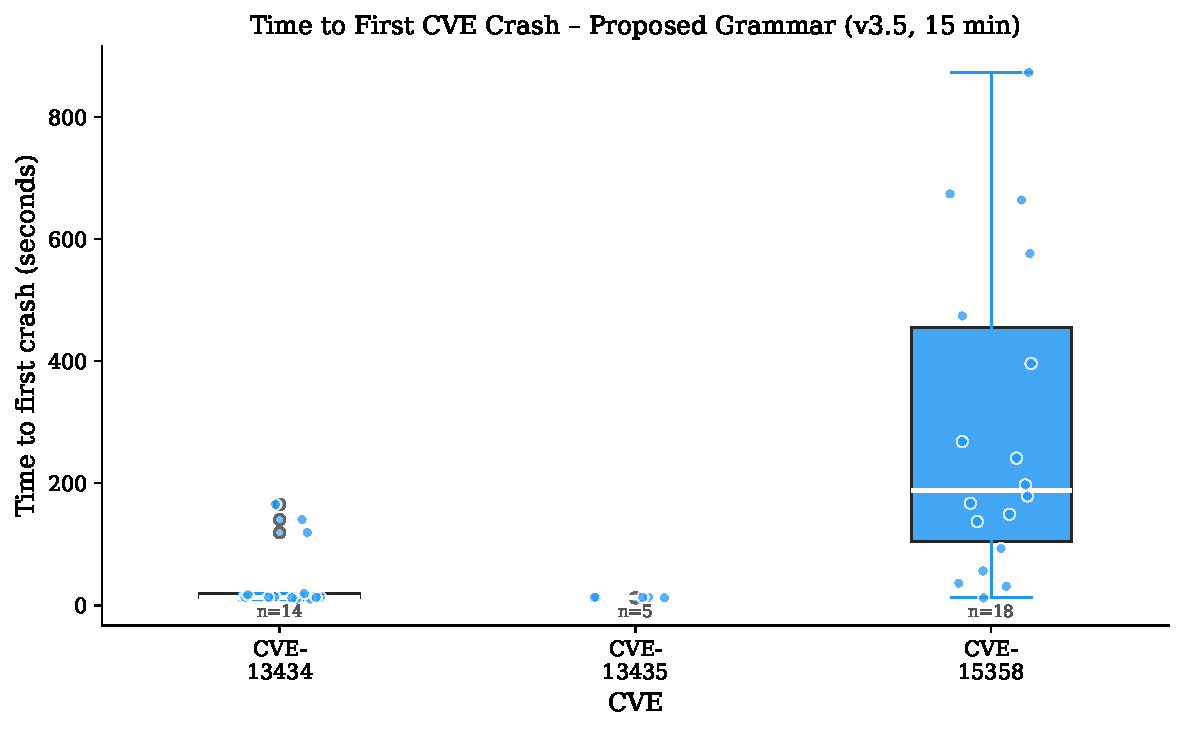
\includegraphics[width=\textwidth]{figures/fig_4_1_time_to_first_cve.pdf}
\caption{Time to first CVE-matching crash across all successful RQ1 runs. Each data point represents one campaign; box plots show the distribution across 5 repetitions.}
\label{fig:time-to-cve}
\end{figure}

These results indicate that the structural-primitives grammar with seed rules achieves reliable CVE rediscovery for 4 of the 5 detectable target CVEs, with the majority of discoveries occurring within the first minutes of campaign execution.


\subsection{RQ2: Bug Detection}
\label{sec:rq2-results}

The compositional grammar (without CVE-specific seed rules, 520 production rules) was evaluated across all four SQLite versions (5 runs per version, 20 campaigns total). Table~\ref{tab:rq2-bugs} presents the 11 distinct bug classes identified through stack-hash deduplication and function-level grouping.

\begin{table}[htbp]
\caption{Bug classes discovered by the compositional grammar (without seed rules) across 20 campaigns. Severity is assigned based on bug type: memory safety violations (HIGH), integer/float overflows (MEDIUM/LOW). Three classes match known CVEs; three are newly discovered; five are known non-CVE bugs.}
\label{tab:rq2-bugs}
\centering
\small
\begin{tabular}{llllcr}
\toprule
\textbf{Class} & \textbf{Bug Type} & \textbf{Sev.} & \textbf{Versions} & \textbf{CVE} & \textbf{Hashes} \\
\midrule
BC001 & Null ptr in \texttt{sqlite3Fts5GetTokenizer} & HIGH & 4 ver. & --- & 4 \\
BC002 & Misaligned in \texttt{WindowUnlinkFromSelect} & HIGH & 3.30.1 & 13871 & 1 \\
BC003 & Int overflow in \texttt{sqlite3\_str\_vappendf} & MED & 3 ver. & 13434 & 6 \\
BC004 & Float cast overflow in \texttt{alsoAnInt} & LOW & 3 ver. & --- & 10 \\
BC006 & Null ptr in \texttt{sqlite3ExprCodeTarget} & HIGH & 3 ver. & --- & 3 \\
BC008 & Null ptr in \texttt{sqlite3Atoi64} & HIGH & 3.30.1 & --- & 2 \\
BC009 & Float cast overflow in \texttt{VdbeMemNumerify} & LOW & 3.32.2 & --- & 2 \\
BC010 & Null ptr in \texttt{sqlite3Select} & HIGH & 3.31.1, 3.32.0 & 9327 & 2 \\
BC011 & Misaligned in \texttt{resetAccumulator} & HIGH & 3.30.1 & --- & 1 \\
BC012 & Null ptr in \texttt{isAuxiliaryVtabOperator} & HIGH & 3.31.1 & --- & 1 \\
BC013 & Misaligned in \texttt{sqlite3ExprCodeTarget} & HIGH & 3.31.1 & --- & 13 \\
\midrule
\multicolumn{5}{l}{\textbf{Total unique hashes}} & \textbf{45} \\
\bottomrule
\end{tabular}
\end{table}

The 11 bug classes decompose into three categories: 3 CVE matches (BC002 matching CVE-2020-13871, BC003 matching CVE-2020-13434, BC010 matching CVE-2020-9327), 5 known non-CVE bugs (BC001, BC004, BC006, BC008, BC009), and 3 newly discovered bugs (BC011, BC012, BC013) that have not been previously reported in the SQLite bug tracker or CVE database.

Table~\ref{tab:rq2-per-run} shows the mean number of distinct bug classes discovered per campaign for each SQLite version.

\begin{table}[htbp]
\caption{Bug class discovery per campaign (mean $\pm$ std across 5 runs) using the compositional grammar without seed rules. The proposed grammar row is \textbf{bolded}.}
\label{tab:rq2-per-run}
\centering
\begin{tabular}{lcccc}
\toprule
\textbf{Grammar} & \textbf{3.30.1} & \textbf{3.31.1} & \textbf{3.32.0} & \textbf{3.32.2} \\
\midrule
\textbf{Compositional (proposed)} & $\mathbf{5.4 \pm 0.5}$ & $\mathbf{5.0 \pm 0.7}$ & $\mathbf{3.4 \pm 0.5}$ & $\mathbf{1.4 \pm 0.9}$ \\
\bottomrule
\end{tabular}
\end{table}

Figure~\ref{fig:bug-breakdown} presents the per-version bug class distribution across all 20 campaigns.

\begin{figure}[htbp]
\centering
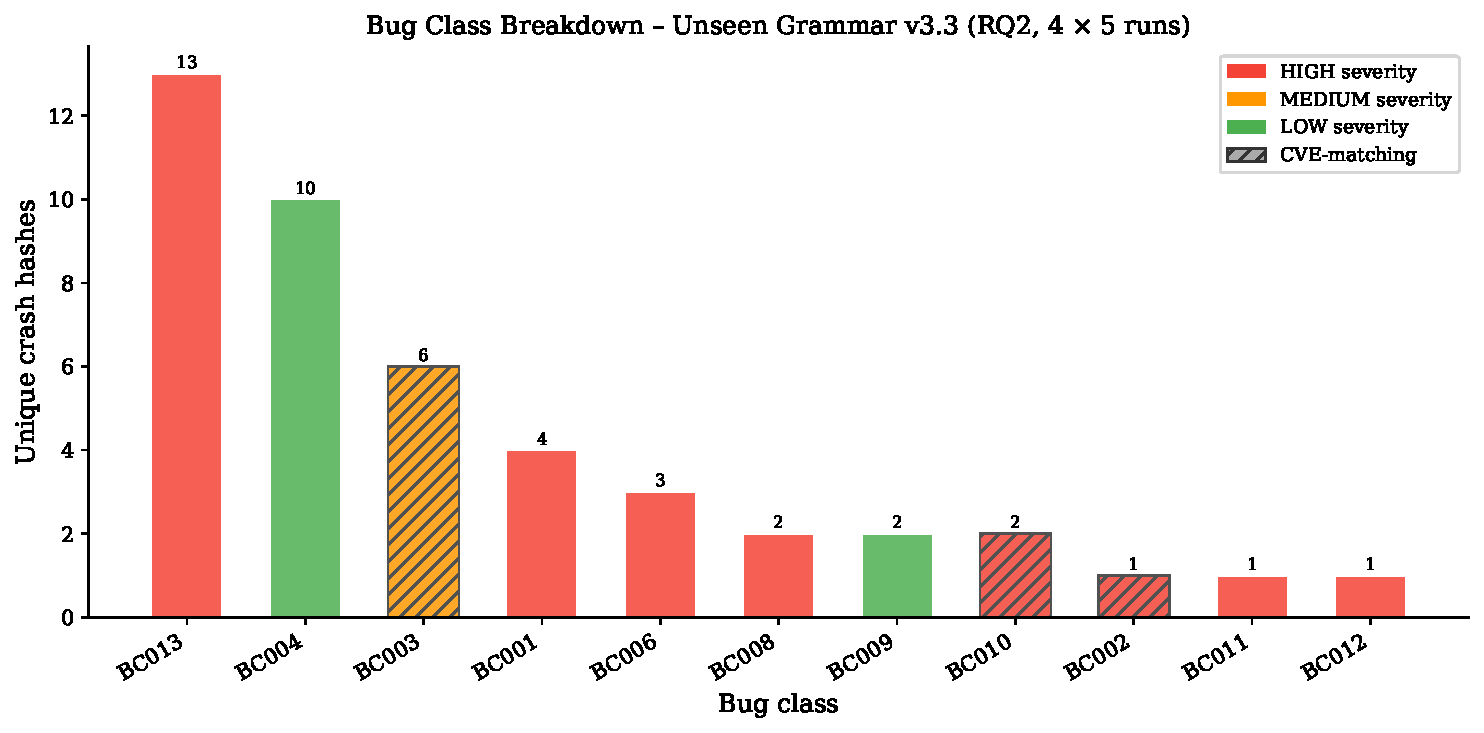
\includegraphics[width=\textwidth]{figures/fig_4_2_bug_class_breakdown.pdf}
\caption{Bug class breakdown across SQLite versions for the compositional grammar (20 campaigns). Each bar segment represents one bug class; height indicates crash count.}
\label{fig:bug-breakdown}
\end{figure}

A notable finding is the compositional discovery of CVE-2020-9327 (BC010). This CVE, which was not triggered by the seed-augmented grammar in RQ1 (0/5 runs on 3.31.1), was found by the compositional grammar without any seed rules --- once on version~3.31.1 (run~4) and four times on version~3.32.0 (runs 3, with 4 crash instances). This demonstrates that the grammar's structural primitives can independently compose the four simultaneous elements required to trigger this CVE (self-referential generated column, view reference, \texttt{coalesce()} call, and \texttt{JOIN} operation), providing evidence for cross-pollination between non-terminals designed for different purposes.


The three newly discovered bug classes merit individual examination:

\paragraph{BC011 --- Misaligned access in \texttt{resetAccumulator}.}
Found exclusively on version~3.30.1 with 13 total crashes and 1 unique hash, this bug occurs in the aggregate function accumulator reset path. Under \texttt{SQLITE\_DEBUG}, freed memory is filled with \texttt{0xAA} bytes, and the subsequent access to the poisoned memory triggers UBSan's misaligned-access diagnostic. The bug is related to but distinct from CVE-2020-13871 (BC002): BC002 crashes during window function \emph{unlinking}, while BC011 crashes during accumulator \emph{reset} --- two separate defects in the window function memory management pipeline.

\paragraph{BC012 --- Null pointer dereference in \texttt{isAuxiliaryVtabOperator}.}
Found on version~3.31.1 with 20 total crashes and 1 unique hash, this bug is a null pointer dereference in the virtual table operator classification logic. It is triggered when the query planner attempts to classify an operator for a virtual table query involving an FTS5 table with certain column configurations. The persistence across all 5 runs on version~3.31.1 (2--6 crashes per run) indicates reliable triggering once the grammar generates the required FTS5 schema and query combination.

\paragraph{BC013 --- Misaligned access in \texttt{sqlite3ExprCodeTarget}.}
Found on version~3.31.1 with 13 total crashes and 13 unique hashes, this bug produces a distinct stack hash for each crash instance, suggesting that many different SQL patterns can trigger the same underlying misaligned memory access in the expression code generator. The 13 unique hashes from 13 crashes indicate that each triggering input exercises a slightly different path through the expression evaluation logic, all converging on the same misaligned pointer dereference.

These results suggest that the compositional grammar discovers a diverse set of bug classes beyond the target CVEs, including 3 previously unreported defects, through cross-pollination between structural primitives designed for different vulnerability patterns.


\subsection{RQ3: Performance Trade-off}
\label{sec:rq3-results}

Table~\ref{tab:rq3-stats} presents the statistical comparison between the proposed grammar and the EBNF baseline across four metrics, using the Mann-Whitney~$U$ test with Cliff's~$d$ effect size. Each cell reports mean $\pm$ standard deviation across 5 runs.

\begin{table}[htbp]
\caption{Statistical comparison: proposed grammar vs EBNF baseline (15-minute campaigns, $n=5$ per cell). Cliff's $d$: large ($|d| \geq 0.474$), medium ($|d| \geq 0.33$), small ($|d| \geq 0.147$). The proposed grammar row is \textbf{bolded} in each metric block.}
\label{tab:rq3-stats}
\centering
\small
\begin{tabular}{llrrrl}
\toprule
\textbf{Metric} & \textbf{Version} & \textbf{Proposed} & \textbf{EBNF} & \textbf{$p$-value} & \textbf{Cliff's $d$} \\
\midrule
\multirow{4}{*}{Unique RCs}
  & 3.30.1 & $\mathbf{215.4 \pm 24.4}$ & $3.6 \pm 2.1$ & 0.008 & $+1.00$ (large) \\
  & 3.31.1 & $\mathbf{170.6 \pm 72.4}$ & $1.0 \pm 0.0$ & 0.004 & $+1.00$ (large) \\
  & 3.32.0 & $\mathbf{139.4 \pm 73.0}$ & $5.0 \pm 6.9$ & 0.020 & $+0.92$ (large) \\
  & 3.32.2 & $\mathbf{296.8 \pm 38.2}$ & $1.0 \pm 0.0$ & 0.008 & $+1.00$ (large) \\
\midrule
\multirow{4}{*}{Edge Cov.}
  & 3.30.1 & $18{,}867 \pm 833$ & $\mathbf{23{,}323 \pm 152}$ & 0.008 & $-1.00$ (large) \\
  & 3.31.1 & $19{,}333 \pm 645$ & $\mathbf{23{,}182 \pm 341}$ & 0.008 & $-1.00$ (large) \\
  & 3.32.0 & $20{,}108 \pm 852$ & $\mathbf{22{,}360 \pm 2{,}886}$ & 0.151 & $-0.60$ (large) \\
  & 3.32.2 & $20{,}953 \pm 525$ & $\mathbf{23{,}811 \pm 166}$ & 0.008 & $-1.00$ (large) \\
\midrule
\multirow{4}{*}{Throughput}
  & 3.30.1 & $76.7 \pm 20.1$ & $\mathbf{196.1 \pm 15.9}$ & 0.008 & $-1.00$ (large) \\
  & 3.31.1 & $56.8 \pm 9.2$ & $\mathbf{182.4 \pm 12.2}$ & 0.008 & $-1.00$ (large) \\
  & 3.32.0 & $71.8 \pm 14.4$ & $\mathbf{241.9 \pm 99.2}$ & 0.012 & $-1.00$ (large) \\
  & 3.32.2 & $103.8 \pm 39.5$ & $\mathbf{182.2 \pm 15.8}$ & 0.016 & $-0.92$ (large) \\
\midrule
\multirow{4}{*}{TTFC (s)}
  & 3.30.1 & $\mathbf{1.8 \pm 0.8}$ & $1.8 \pm 1.3$ & 0.821 & $+0.12$ (negl.) \\
  & 3.31.1 & $\mathbf{1.2 \pm 0.4}$ & $1.2 \pm 0.4$ & 1.000 & $0.00$ (negl.) \\
  & 3.32.0 & $1.6 \pm 0.5$ & $\mathbf{1.0 \pm 0.0}$ & 0.101 & $+0.60$ (large) \\
  & 3.32.2 & $3.4 \pm 3.0$ & $\mathbf{1.8 \pm 1.1}$ & 0.502 & $+0.28$ (small) \\
\bottomrule
\end{tabular}
\end{table}

The results reveal a clear trade-off between structural complexity and raw throughput. The EBNF baseline achieves $1.8\times$--$3.4\times$ higher throughput (mean 200.7 executions per second vs 77.3 for the proposed grammar) and $1.1\times$--$1.2\times$ higher edge coverage (mean 23{,}169 vs 19{,}815 edges). However, the proposed grammar discovers $28\times$--$297\times$ more unique root causes per campaign (mean 205.6 vs 2.6), with large effect sizes ($d \geq 0.92$, $p < 0.05$) on all four versions.

Time to first crash (TTFC) shows no statistically significant difference between the two grammars on any version ($p > 0.05$ on all four), indicating that both grammars find their first crash within seconds of campaign start. The throughput disadvantage of the proposed grammar does not translate into a delay in initial crash discovery.

Figure~\ref{fig:coverage-growth} shows the edge coverage growth over the 15-minute campaign duration for both grammars. The EBNF baseline reaches higher absolute coverage due to its higher throughput and broader syntactic variety, but the proposed grammar's coverage growth rate suggests that it explores a smaller but more vulnerability-relevant subset of the code.

\begin{figure}[htbp]
\centering
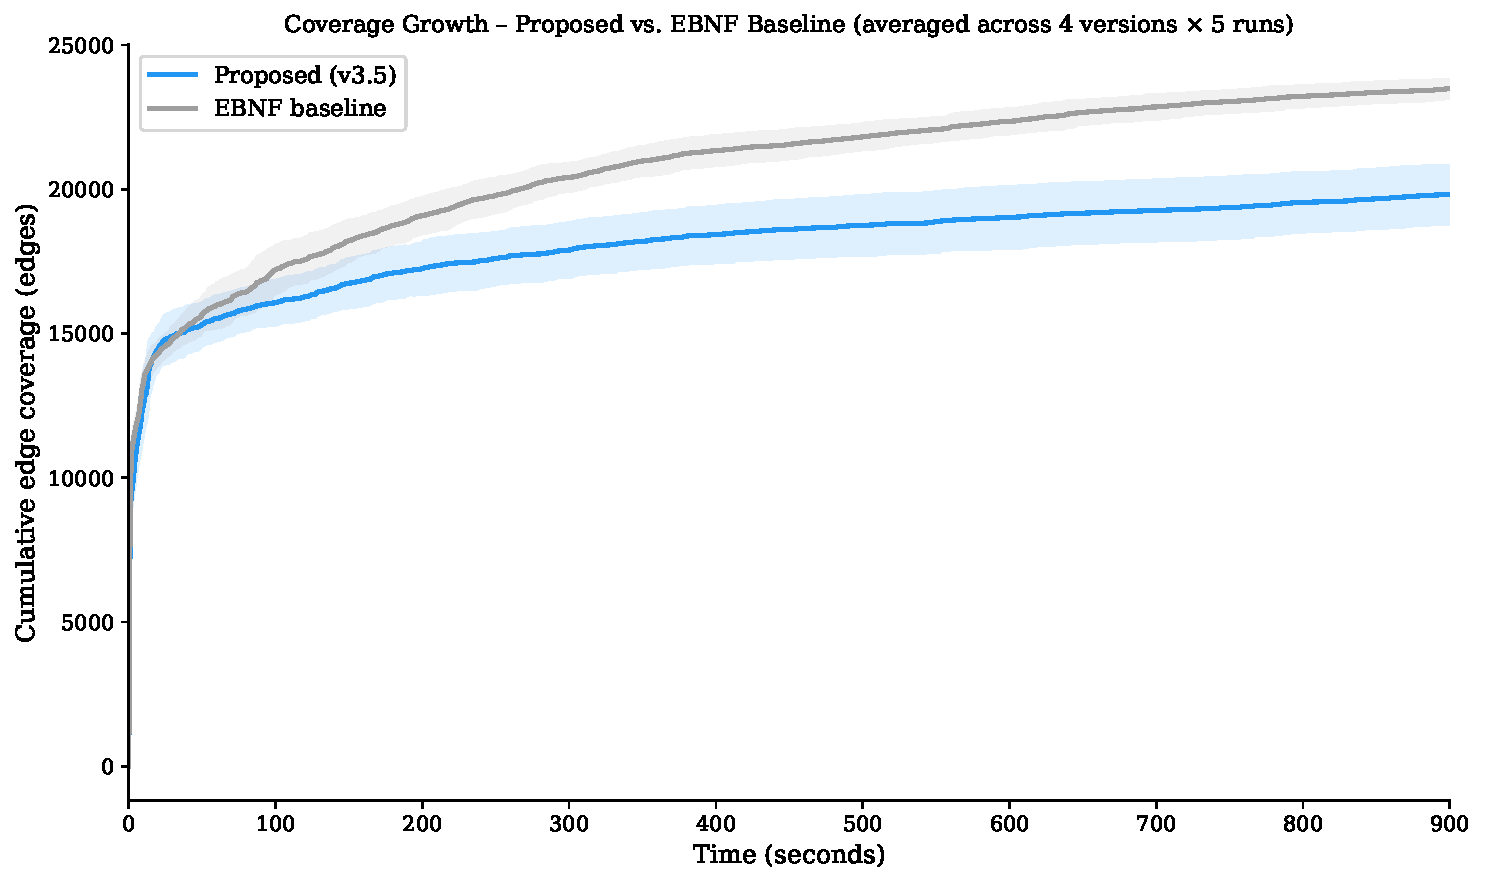
\includegraphics[width=\textwidth]{figures/fig_4_3_coverage_growth.pdf}
\caption{Edge coverage growth over time: proposed grammar vs EBNF baseline. Solid lines show mean across 5 runs; shaded bands show $\pm$1 standard deviation.}
\label{fig:coverage-growth}
\end{figure}

Figure~\ref{fig:throughput} presents the throughput comparison across all four versions. The EBNF grammar's simpler production rules generate shorter SQL inputs, resulting in faster execution per test case.

\begin{figure}[htbp]
\centering
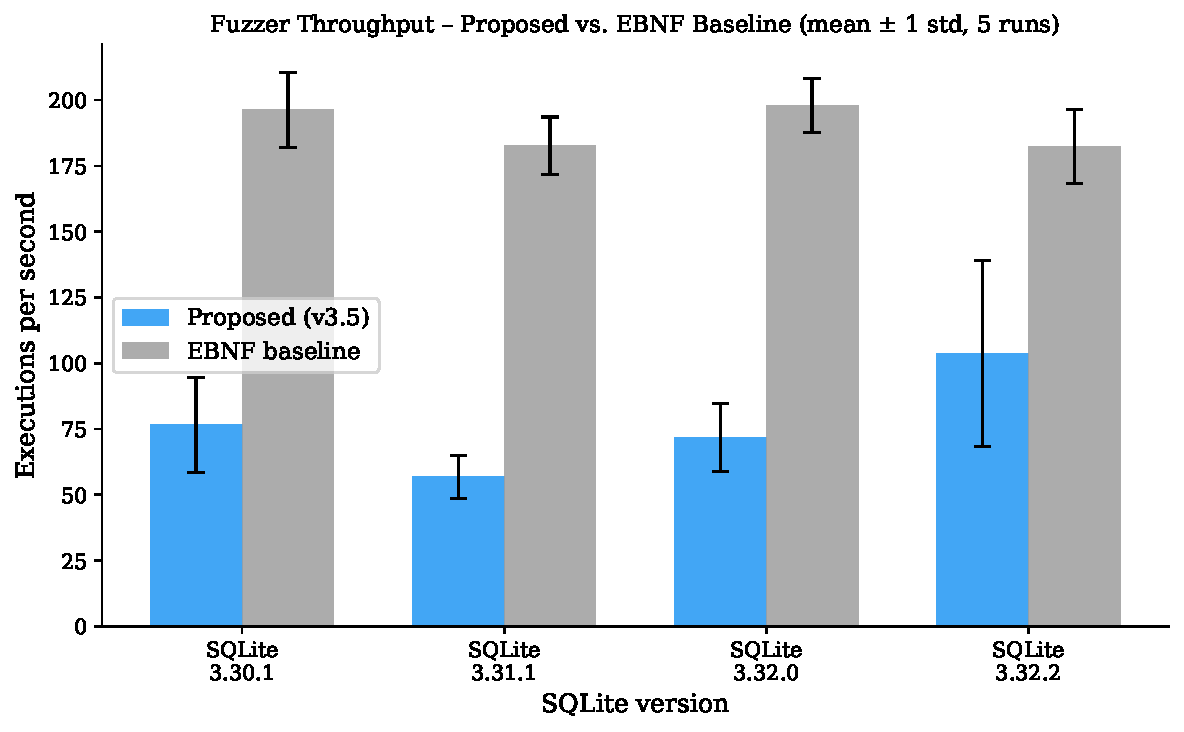
\includegraphics[width=\textwidth]{figures/fig_4_4_throughput.pdf}
\caption{Throughput comparison (executions per second) between the proposed grammar and EBNF baseline across 4 SQLite versions. Error bars show $\pm$1 standard deviation.}
\label{fig:throughput}
\end{figure}

Figure~\ref{fig:ttfc} shows the time-to-first-crash distribution for both grammars, confirming the negligible difference in initial crash discovery latency.

\begin{figure}[htbp]
\centering
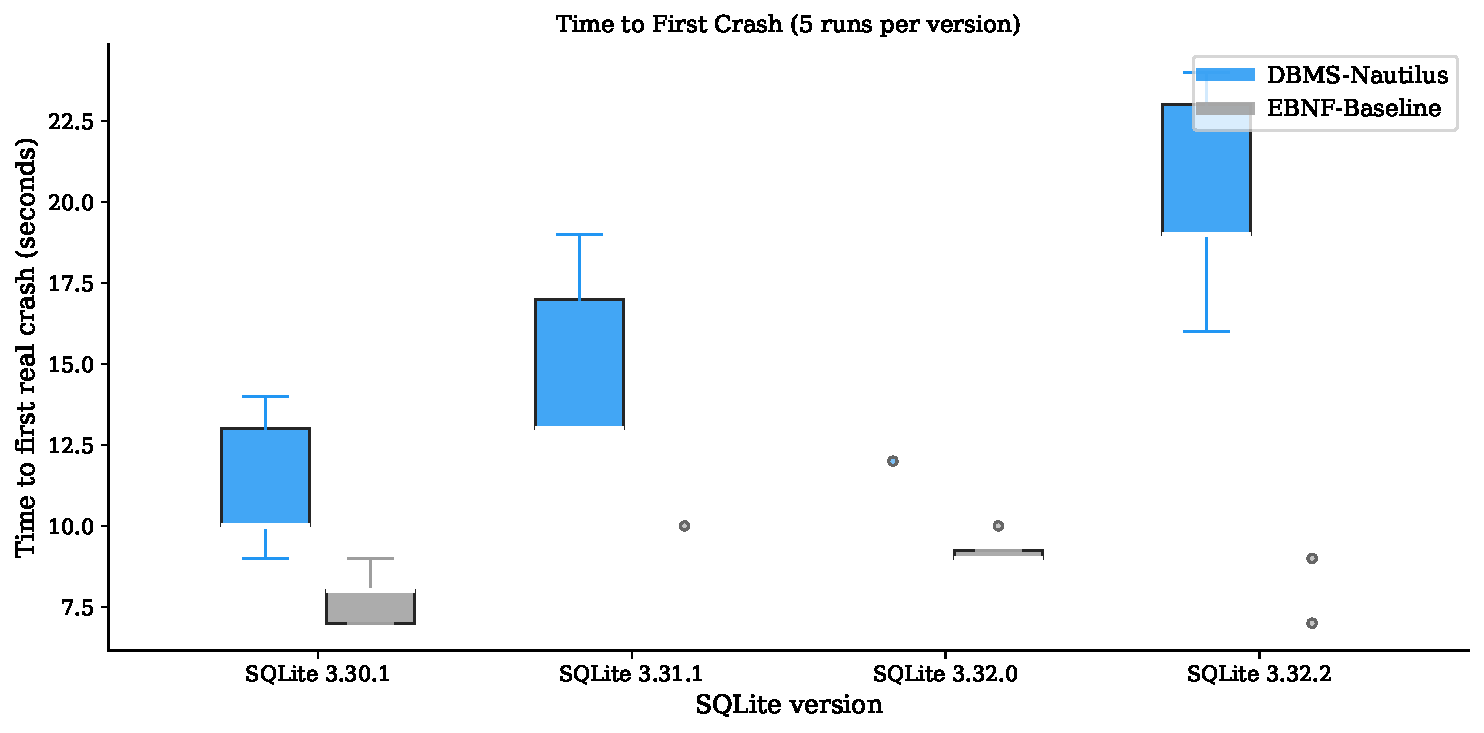
\includegraphics[width=\textwidth]{figures/fig_4_5_time_to_first_crash.pdf}
\caption{Time to first crash (seconds): proposed grammar vs EBNF baseline. No statistically significant difference on any version ($p > 0.05$).}
\label{fig:ttfc}
\end{figure}

These results indicate that the proposed grammar sacrifices throughput and edge coverage breadth in exchange for dramatically higher crash diversity, suggesting that structural complexity in grammar design redirects fuzzing effort toward vulnerability-relevant code paths at the cost of raw execution speed.


\section{Analysis and Discussion}
\label{sec:discussion}

\subsection{Qualitative Analysis}
\label{sec:qualitative}

The 11 bug classes discovered by the compositional grammar (RQ2) can be organized into three groups based on their relationship to the grammar's design intent:

\emph{CVE-matching bugs} (3 classes, 27.3\% of total). BC002 (CVE-2020-13871), BC003 (CVE-2020-13434), and BC010 (CVE-2020-9327) are rediscoveries of known CVEs through compositional generation of structural primitives. These validate the grammar's primary design objective: encoding vulnerability-relevant patterns that can reconstruct CVE-triggering inputs without embedding proof-of-concept strings.

\emph{Cross-pollination bugs} (5 classes, 45.5\% of total). BC001 (FTS5 tokenizer null pointer), BC004 (float cast overflow in \texttt{alsoAnInt}), BC006 (expression code generator null pointer), BC008 (numeric conversion null pointer), and BC009 (VDBE numerify float cast overflow) are bugs found through structural primitives designed for specific CVEs but which also exercise adjacent code paths. The \texttt{Boundary-Func-Call} non-terminal, designed to trigger CVE-2020-13434's integer overflow, also produces boundary float values that trigger BC004 and BC009. The FTS schema template, designed to create virtual table contexts for CVE-targeting queries, triggers BC001 through malformed tokenizer configurations.

\emph{Emergent bugs} (3 classes, 27.3\% of total). BC011 (accumulator reset misalignment), BC012 (virtual table operator null pointer), and BC013 (expression code target misalignment) were discovered through grammar patterns that were not explicitly designed for any specific vulnerability. BC011 emerges from the interaction between window function rules and aggregate function processing. BC012 emerges from FTS5 virtual table queries with specific column configurations. BC013 produces 13 unique hashes from 13 crashes, indicating a rich space of triggering patterns for the same underlying defect.

\subsection{Comparison with Baseline}
\label{sec:comparison}

Table~\ref{tab:comparison-summary} summarizes the key metrics across both grammars from the RQ3 evaluation.

\begin{table}[htbp]
\caption{Overall comparison: proposed grammar vs EBNF baseline (mean across all versions and runs). The proposed grammar row is \textbf{bolded}.}
\label{tab:comparison-summary}
\centering
\begin{tabular}{lrr}
\toprule
\textbf{Metric} & \textbf{Proposed} & \textbf{EBNF} \\
\midrule
Unique root causes per campaign & $\mathbf{205.6 \pm 79.7}$ & $2.6 \pm 3.8$ \\
Edge coverage per campaign & $19{,}815 \pm 782$ & $\mathbf{23{,}169 \pm 1{,}441}$ \\
Throughput (execs/sec) & $77.3 \pm 23.6$ & $\mathbf{200.7 \pm 53.3}$ \\
TTFC (seconds) & $\mathbf{2.0 \pm 1.7}$ & $1.5 \pm 0.9$ \\
\bottomrule
\end{tabular}
\end{table}

The proposed grammar discovers $79\times$ more unique root causes per campaign than the EBNF baseline (205.6 vs 2.6), at the cost of 61.5\% lower throughput and 14.5\% lower edge coverage. This asymmetry suggests that the EBNF grammar's higher throughput and coverage are ``shallow'' --- it executes more inputs and touches more edges, but the additional coverage is concentrated in non-vulnerable code paths. The proposed grammar's structural complexity directs generation toward the subset of SQL constructs that exercise vulnerability-relevant code, producing denser crash discovery per execution despite the lower throughput.

The EBNF baseline found 4 distinct function-level bug classes (excluding debug-assert-only \texttt{unknown} crashes): \texttt{sqlite3Fts5GetTokenizer} (BC001), \texttt{sqlite3WindowUnlinkFromSelect} (BC002), \texttt{alsoAnInt} (BC004), and \texttt{sqlite3WindowListDelete}. The proposed grammar found these same 4 classes plus 2 additional ones: \texttt{sqlite3ExprCodeTarget} (BC006) and \texttt{sqlite3\_str\_vappendf} (BC003/CVE-2020-13434). The EBNF grammar's inability to trigger CVE-2020-13434 (which requires a \texttt{printf()} call with a specific format specifier and boundary integer) demonstrates that certain bug classes require domain-specific structural patterns that generic grammar specifications cannot express.

An interesting observation concerns CVE-2020-13871 (BC002). The EBNF baseline found this CVE on version~3.30.1 in 4 out of 5 runs, while the proposed grammar found it on 3.30.1 in all compositional (RQ2) campaigns and confirmed it via seed-derived crashes on 3.32.2 in 4 out of 5 RQ1 runs. This CVE's discovery by the EBNF grammar indicates that the window function code path containing this use-after-free is reachable even through generic SQL generation, likely because window functions are a standard SQL construct that any comprehensive grammar will exercise.

\subsection{Failure Cases and Limitations}
\label{sec:limitations}

At least four concrete limitations of the proposed approach were identified during the evaluation:

\begin{enumerate}
  \item \textbf{Oracle limitation for non-crash bugs.} CVE-2019-19646 causes an infinite loop rather than a crash. The ASan/UBSan oracle detects only memory safety violations and undefined behavior; it cannot detect non-termination, incorrect query results, or other logic bugs. Detecting such bugs would require a timeout oracle with non-termination classification, or a differential testing oracle comparing outputs against a reference implementation.

  \item \textbf{Combinatorial explosion for multi-element CVEs.} CVE-2020-9327 requires four simultaneous structural elements in a single generated tree (self-referential generated column, view, \texttt{coalesce()}, and \texttt{JOIN}). Despite a dedicated seed rule, this CVE was not triggered in 5 RQ1 runs on version~3.31.1. The joint probability of four independent non-terminals co-occurring decreases multiplicatively, and the 15-minute campaign duration may be insufficient for these rare combinations. The compositional discovery in RQ2 (1 instance across 20 campaigns) confirms both the feasibility and the rarity of this conjunction.

  \item \textbf{Context-free grammar cannot enforce semantic validity.} The grammar is context-free and cannot enforce type correctness, referential integrity, or valid column count matching between \texttt{INSERT} values and table definitions. Semantically invalid SQL statements are generated and immediately rejected by SQLite's parser or query planner, consuming execution time without contributing to coverage. The throughput gap between the proposed grammar (77.3 execs/sec) and the EBNF baseline (200.7 execs/sec) is partially attributable to the proposed grammar generating longer, more complex inputs that take more time to parse and reject.

  \item \textbf{Manual CVE analysis dependency.} The structural-primitive methodology requires manual expertise to identify which SQL constructs are relevant to each vulnerability. The effectiveness of the approach depends on the quality of this analysis: if a critical structural pattern is missed or incorrectly characterized, the corresponding grammar rules will be absent or ineffective. Automating this analysis --- for example, through differential code analysis between patched and unpatched versions --- is an open research question.
\end{enumerate}

\subsection{Threats to Validity}
\label{sec:threats}

\paragraph{Internal validity.}
Stack-hash deduplication using the top 5 frames is a heuristic that may both over-count and under-count bug classes. Over-counting occurs when two manifestations of the same root cause crash through different call paths; under-counting occurs when distinct bugs crash through the same 5-frame sequence. The \texttt{SQLITE\_DEBUG} build flag introduces an additional confound: it fills freed memory with \texttt{0xAA} bytes, causing use-after-free bugs to manifest as misaligned-access diagnostics rather than heap-use-after-free reports. This was addressed through no-debug harness replay for CVE confirmation (see Table~\ref{tab:cve-rediscovery}), but may affect the classification accuracy of non-CVE bug classes. Campaign durations of 15~minutes may miss bugs requiring longer exploration or rarer compositional combinations; however, extending campaigns introduces diminishing returns in coverage-guided fuzzing.

\paragraph{External validity.}
All experiments target a single DBMS --- SQLite~\citep{sqlite} --- with a single input language (SQL). SQLite is an embedded database with a compact codebase (${\sim}$150{,}000 lines of C), and its bug landscape may not be representative of larger server-based systems such as MySQL or PostgreSQL. The comparison uses a single baseline grammar (EBNF) rather than multiple baselines or existing fuzzing tools such as SQLsmith~\citep{sqlsmith} or Squirrel~\citep{squirrel}. Direct comparison with these tools was not feasible because they use fundamentally different fuzzing strategies (query-plan-guided generation for SQLsmith, AST-level mutation for Squirrel) that cannot be isolated to a grammar-only comparison. The EBNF baseline isolates the effect of grammar design by holding all other variables constant.

\paragraph{Construct validity.}
The 80\% fidelity threshold for CVE signature matching is an arbitrary cutoff. A higher threshold would reduce false positive matches but might miss legitimate rediscoveries where the stack trace differs due to compiler optimizations or ASan instrumentation overhead. The sanitizer oracle misses entire categories of bugs: logic bugs producing incorrect results without undefined behavior, and denial-of-service bugs causing non-termination without crashing. Edge coverage as measured by the AFL-style bitmap is subject to hash collisions, where distinct edges map to the same bitmap byte, potentially causing the fuzzer to miss coverage-increasing inputs.

\subsection{Summary}
\label{sec:summary}

The experimental evaluation demonstrates three principal findings. First, the proposed grammar with seed rules reliably rediscovers 4 out of 5 detectable CVEs across 20 campaigns, confirming that domain-knowledge-driven grammar engineering can reconstruct CVE-triggering inputs from independently encoded structural primitives (RQ1). Second, the compositional grammar without seed rules discovers 11 distinct bug classes --- including 3 previously unreported defects and 3 CVE matches found without dedicated seeds --- demonstrating that structural primitives designed for specific CVEs cross-pollinate to exercise adjacent vulnerable code paths (RQ2). Third, the proposed grammar sacrifices throughput ($2.6\times$ slower) and edge coverage (14.5\% lower) in exchange for $79\times$ more unique root causes per campaign, indicating that structural complexity redirects fuzzing effort toward vulnerability-relevant code at the cost of raw execution speed (RQ3). The EBNF baseline's CVE rediscovery was limited to CVE-2020-13871 on version~3.30.1, which requires only standard window function syntax reachable through generic SQL generation.
